\documentclass{article}

\usepackage{graphicx} % Required for the inclusion of images
\usepackage{amsmath} % Required for some math elements
\usepackage{hyperref}
\usepackage[numbers,sort]{natbib}
\usepackage[russian,english]{babel}
\usepackage[T2A]{fontenc}
\usepackage{placeins}
\usepackage{hyperref}
\usepackage[figurename=Рисунок]{caption}
\graphicspath{ {./figs/} }
\setlength\parindent{0pt} % Removes all indentation from paragraphs
\renewcommand{\labelenumi}{\alph{enumi}.} % Make numbering in the enumerate environment by letter
\title{Адаптивное и робастное управление \\ Работа №5(8) \\ Отчет В-17} % Title
\author{Кирилл Лалаянц \\ Егор Прокопов} % Author name
\date{\today} % Date for the report

\begin{document}

\maketitle % Insert the title, author and date

\begin{center}
\begin{tabular}{l r}
%Date Performed: & January 1, 2012 \\ % Date the experiment was performed
% Выполнили: & Кирилл Лалаянц \\ % Partner names
% &Прокопов Егор \\
Преподаватель: & Козачёк О.А. % Instructor/supervisor
\end{tabular}
\end{center}
\newpage
% \begin{abstract}
% Abstract text
% \end{abstract}

\section{Цель работы}

Освоение метода расширенной ошибки в задачах
адаптивного управления по выходу.

\section{Выполнение}
\[
\begin{cases}
    y_m = \frac{k_0}{K_M(s)}[g(t)] \\
    y = \frac{1}{K_M(s)}[k_0 g - \psi^T \omega + b_m u] + \delta(t) \\
    u = \frac{1}{\hat{b}_m}(-\hat{\psi}_p^T \omega + k_0 g(t)) \\
    \dot {\hat{\psi}}_p^T = \gamma \Gamma \frac{\bar \omega_p}{1 + \bar \omega_p^T \bar \omega_p} \hat \varepsilon\\
    \hat \varepsilon = \varepsilon - \hat{\psi}_p^T \bar \omega_p + \frac{1}{K_M(s)}[ \hat{\psi}_p^T \omega_p] \\
    \hat{\psi}_p^T = [\hat \psi ~~ \hat b_m] \\
    \omega^T = [\nu_1 ~~ \nu_2 ~~ y] \\
    \omega_p^T = -[\omega^T ~~ u] \\
    \dot \nu_1 = \Lambda \nu_1 + e_{n-1}u \\
    \dot \nu_2 = \Lambda \nu_2 + e_{n-1}y \\
    b_m(t) > b_{min} \text{ -- известно}; 
\end{cases}
\]

При моделировании в Simulink использовались следующие значения параметров: 
\begin{itemize}
  \item \(a_1 = 6\); \(a_0 = 9\);
  \item \(b_0 = 2\);
  \item \(k_{M_1} = 10\); \(k_{M_0} = 25\);
  \item \(k_0 = 7\);
  \item \(\Lambda = -k_0\);
  \item \(m = 1; ~ b_m = b_1\)
  \item \(y_m(0) = 0; y_m(0) = 0.4\).
\end{itemize}

\newpage
\subsection{Управление 0}
Сначала было проведено моделирование при \(g(t) = 0\). 
% Так как не выполняется условие незатухающего возбуждения, параметрическая ошибка \(\tilde \theta = \theta - \hat \theta\) и норма ошибки вектора состояния \(||\hat x - x||\) не сходятся к 0. 
Результаты представлены на рис. \ref{fig:1_epsilon} - \ref{fig:1_psi0_psi_p_hat_3}.

Как видно, ошибка слежения сводится к 0, все параметры ограничены.
\begin{figure}[h!]
  \centering
  \includegraphics[width=0.5\textwidth]{figs/0_epsilon.png}
  \caption{График ошибки слежения линейного объекта при \(g(t) = 0\).} 
  \label{fig:1_epsilon}
\end{figure}
\begin{figure}[h!]
  \centering
  \includegraphics[width=0.5\textwidth]{figs/0_u.png}
  \caption{График сигнала настраиваемого регулятора линейного объекта при \(g(t) = 0\).} 
  \label{fig:1_u}
\end{figure}
\begin{figure}[h!]
  \centering
  \includegraphics[width=0.5\textwidth]{figs/0_psi_p_hat_0.png}
  \caption{График первого элемента вектора параметров \(\hat{\psi}_p\) при \(g(t) = 0\).} 
  \label{fig:1_psi0_psi_p_hat_0}
\end{figure}
\begin{figure}[h!]
  \centering
  \includegraphics[width=0.5\textwidth]{figs/0_psi_p_hat_1.png}
  \caption{График второго элемента вектора параметров \(\hat{\psi}_p\) при \(g(t) = 0\).} 
  \label{fig:1_psi0_psi_p_hat_1}
\end{figure}
\begin{figure}[h!]
  \centering
  \includegraphics[width=0.5\textwidth]{figs/0_psi_p_hat_2.png}
  \caption{График третьего элемента вектора параметров \(\hat{\psi}_p\) при \(g(t) = 0\).} 
  \label{fig:1_psi0_psi_p_hat_2}
\end{figure}
\begin{figure}[h!]
  \centering
  \includegraphics[width=0.5\textwidth]{figs/0_psi_p_hat_3.png}
  \caption{График четвертого элемента вектора параметров \(\hat{\psi}_p\) при \(g(t) = 0\).} 
  \label{fig:1_psi0_psi_p_hat_3}
\end{figure}
\FloatBarrier
\newpage

\subsection{Управление не 0}
Было проведено моделирование при \(g(t) = sign(\sin(0.5t))\). 

Результаты представлены на рис. \ref{fig:2_epsilon} - \ref{fig:2_psi0_psi_p_hat_3}.

Как видно, ошибка слежения сводится к 0, все параметры ограничены.
\begin{figure}[h!]
  \centering
  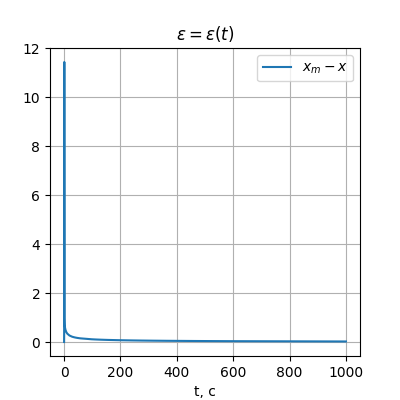
\includegraphics[width=0.5\textwidth]{figs/1_epsilon.png}
  \caption{График ошибки слежения линейного объекта при \(g(t) = sign(\sin(0.5t))\).} 
  \label{fig:2_epsilon}
\end{figure}
\begin{figure}[h!]
  \centering
  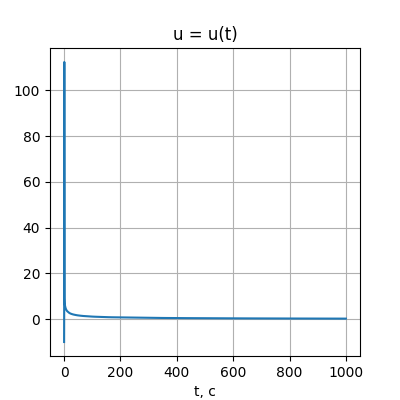
\includegraphics[width=0.5\textwidth]{figs/1_u.png}
  \caption{График сигнала настраиваемого регулятора линейного объекта при \(g(t) = sign(\sin(0.5t))\).} 
  \label{fig:2_u}
\end{figure}
\begin{figure}[h!]
  \centering
  \includegraphics[width=0.5\textwidth]{figs/1_psi_p_hat_0.png}
  \caption{График первого элемента вектора параметров \(\hat{\psi}_p\) при \(g(t) = sign(\sin(0.5t))\).} 
  \label{fig:2_psi0_psi_p_hat_0}
\end{figure}
\begin{figure}[h!]
  \centering
  \includegraphics[width=0.5\textwidth]{figs/1_psi_p_hat_1.png}
  \caption{График второго элемента вектора параметров \(\hat{\psi}_p\) при \(g(t) = sign(\sin(0.5t))\).} 
  \label{fig:2_psi0_psi_p_hat_1}
\end{figure}
\begin{figure}[h!]
  \centering
  \includegraphics[width=0.5\textwidth]{figs/1_psi_p_hat_2.png}
  \caption{График третьего элемента вектора параметров \(\hat{\psi}_p\) при \(g(t) = sign(\sin(0.5t))\).} 
  \label{fig:2_psi0_psi_p_hat_2}
\end{figure}
\begin{figure}[h!]
  \centering
  \includegraphics[width=0.5\textwidth]{figs/1_psi_p_hat_3.png}
  \caption{График четвертого элемента вектора параметров \(\hat{\psi}_p\) при \(g(t) = sign(\sin(0.5t))\).} 
  \label{fig:2_psi0_psi_p_hat_3}
\end{figure}
\FloatBarrier
\newpage
\FloatBarrier
\newpage
\section{Заключение}
Закон адаптивного управления обеспечивает следующие свойства в
замкнутой системе
\begin{itemize}
  \item все сигналы ограничены;
  \item \( \varepsilon \rightarrow 0 \) асимптотически;
  \item \( \tilde \psi_p \rightarrow 0 \), если \(\bar \omega_p\) удовлетворяет условию неисчезающего возбуждения (зависит от частотной насыщенности сигнала задания \(g\));
\end{itemize}
Моделирование в среде Simulink подтвердило данные свойства.
\end{document}
